\documentclass[12pt]{article}
\usepackage{amsmath}
\usepackage{graphicx,geometry}
\usepackage{array}
\geometry{margin=1in}
\usepackage{setspace}
\usepackage{titling}
\setlength{\parskip}{0.5em}

\begin{document}
\begin{minipage}{0.45\textwidth}
  
\includegraphics[width=\linewidth]{Logo.png}
\end{minipage}
\hfill
\begin{minipage}{0.45\textwidth}
  \raggedleft
  \textbf{Name: Surabhi P}\\
  \textbf{Id: COMETFWC032}\\
  \textbf{Date: 29 August 2025}
\end{minipage}

\vspace{1cm}

\begin{center}
    {\LARGE \textbf{GATE Question solution using assembly}}\\[1em]
\end{center}

\section*{Question}
\begin{center}
    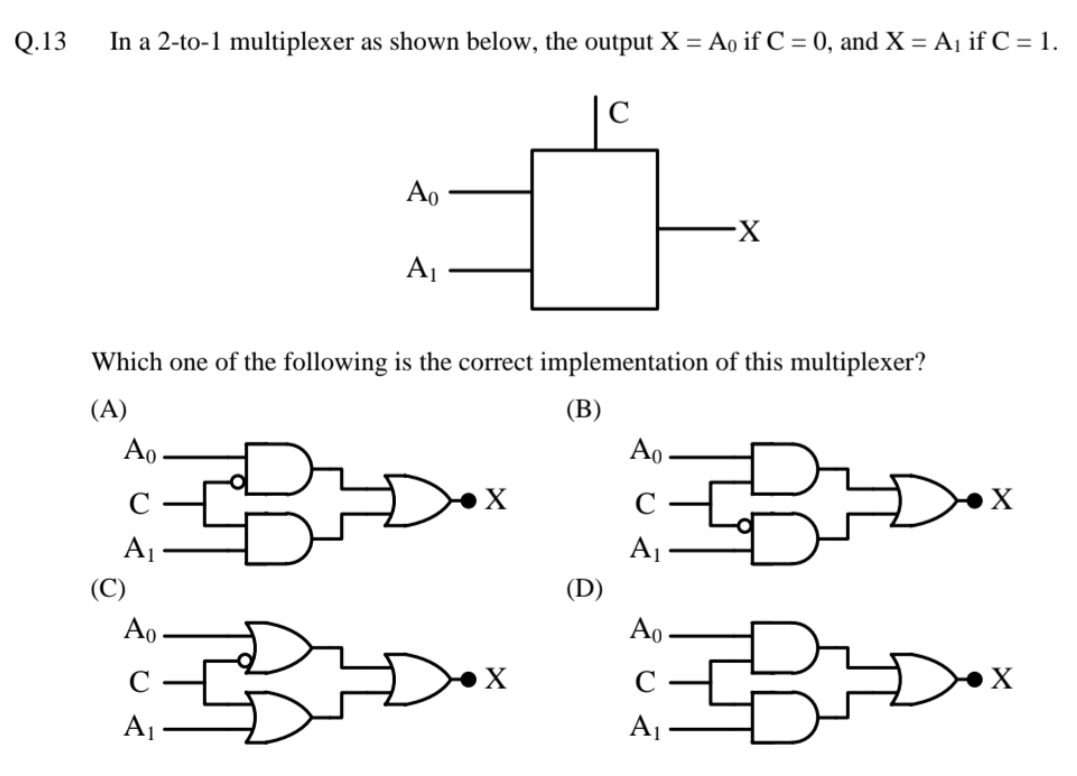
\includegraphics[width=0.6\textwidth]{mquestion.png}
\end{center}

\section*{Solution}
The 2-to-1 multiplexer can be realized using the equation:
\[
X = A_1C + A_0\overline{C}
\]
This requires two AND gates and one OR gate. One AND gate gets inputs $A_1$ and $C$, another gets $A_0$ and the complement of $C$, and their outputs are ORed together.

\section*{Truth Table}
\begin{center}
\begin{tabular}{|c|c|c|c|}
\hline
$A_1$ & $A_0$ & $C$ & $X$ \\
\hline
0 & 0 & 0 & 0 \\
0 & 1 & 0 & 1 \\
1 & 0 & 1 & 1 \\
1 & 1 & 1 & 1 \\
0 & 1 & 1 & 0 \\
1 & 0 & 0 & 0 \\
\hline
\end{tabular}
\end{center}

\section*{AVR Assembly Steps Using Termux}
\begin{enumerate}
    \item Install Termux and AVR tools:
    \begin{verbatim}
pkg update
pkg install proot-distro git curl nano
proot-distro install debian
proot-distro login debian
apt update
apt install avra avrdude
    \end{verbatim}

    \item Write the assembly code implementing $X = A_1C + A_0\overline{C}$, where $A_1 \leftarrow$ PD3, $A_0 \leftarrow$ PD2, $C \leftarrow$ PD4, and $X \rightarrow$ PB5.
    \item Assemble to hex:
    \begin{verbatim}
avra mux.asm
    \end{verbatim}
    \item Connect Arduino to Android via USB OTG.
    \item Upload hex file:
    \begin{verbatim}
avrdude -p m328p -c arduino -P /dev/ttyACM0 -b 115200 -U flash:w:mux.hex
    \end{verbatim}
    \item Wire respective pins to switch inputs and PB5 to observe output.
\end{enumerate}

\section*{Conclusion}
The 2-to-1 multiplexer was implemented using the formula $X = A_1C + A_0\overline{C}$ in AVR assembly code. The truth table validates that the logic gates yield the correct output for all possible input combinations. The project demonstrates how digital logic can be programmed, assembled, and executed directly on an Arduino via Termux on Android.

\end{document}
